\documentclass[11pt,aspectratio=169]{beamer}

% Packages
\usepackage[utf8]{inputenc}
\usepackage{amsmath,amssymb,amsthm}
\usepackage{graphicx}
\usepackage{booktabs}
\usepackage{hyperref}
\usepackage{algorithmic}
\usepackage{algorithm}
\usepackage{xcolor}
\usepackage{tikz}
\usetikzlibrary{arrows.meta, positioning, shapes.geometric}

% Theme
\usetheme{Madrid}
\usecolortheme{default}

% Custom colors
\definecolor{highlight}{RGB}{200,50,50}
\definecolor{contribution}{RGB}{30,120,180}

% Title Information
\title[Learning Capabilities in RL]{What are Capabilities?\\How Can RL Agents Use Their Own Capabilities While Learning?}
\subtitle{Learning a Mathematical Capability Function to Avoid Exploration Limitations}
\author{}
\date{\today}

\begin{document}

% ============================================================================
% SLIDE 1: Title
% ============================================================================
\begin{frame}
    \titlepage
\end{frame}

% ============================================================================
% SLIDE 2: Motivation
% ============================================================================
\begin{frame}{Motivation: Why Learn Capabilities?}
    \textbf{The Problem:} Standard RL agents assume all actions $a \in \mathcal{A}$ are feasible at every state $s$. They must \textit{attempt} every infeasible action to discover it yields comparitively lower reward.

    \vspace{0.4cm}
    \textbf{Our Perspective:} Learning a capability function shifts the paradigm beyond just maximizing rewards:

    \begin{itemize}
        \item \textbf{Avoid unnecessary exploration} — the agent never wastes samples on  less meaningfull actions (may be physical or environmental constraints).
        \item \textbf{Induce implicit safety} — Agnostically limiting dangerous or infeasible actions acts as a safety mechanism without requiring explicit constraint specification with respect to a particular environment or agent capabilities and acts.
        \item \textbf{Improve reward acquisition} — by shrinking the effective action space at each state, the agent converges faster to high-reward policies.
    \end{itemize}

    \vspace{0.3cm}
    \textit{Can we learn a mathematical function that tells the agent which actions lie within its capability at any given state?}
\end{frame}

% ============================================================================
% SLIDE 3: The Capability Function
% ============================================================================
\begin{frame}{The Capability Function $\phi$}
    We define a \textbf{capability function} that maps a state to feasibility logits over the entire action space:
    \begin{equation}
        \phi_\theta: \mathcal{S} \rightarrow \mathbb{R}^{|\mathcal{A}|}
    \end{equation}

    For each action $a_i$, the output $\phi_\theta(s)_i$ represents the predicted probability that action $a_i$ is \textbf{infeasible} at state $s$:
    \begin{equation}
        P(\text{infeasible} \mid s, a_i) = \sigma\big(\phi_\theta(s)_i\big)
    \end{equation}

    \textbf{Integration with the RL policy} (Post-Posed Masking):
    \begin{equation}
        \pi_{\text{capable}}(a \mid s) \propto \pi_{\text{base}}(a \mid s) \cdot \big(1 - \sigma(\phi_\theta(s)_a)\big)
    \end{equation}

    The base policy $\pi_{\text{base}}$ (DQN, PPO, SAC) is \textit{unaware} of constraints. The capability function $\phi_\theta$ acts as an external post-posed filter, filtering infeasible actions from the policy's output.
\end{frame}

% ============================================================================
% SLIDE 4: How to Learn Phi
% ============================================================================
\begin{frame}{How to Learn the Capability Function?}
    Acquiring $\phi_\theta(s)$ presents a fundamental challenge:

    \vspace{0.3cm}
    \textbf{Approach 1: Mathematical Derivation}
    \begin{itemize}
        \item Requires a priori expert knowledge of the transition dynamics $\mathcal{T}(s, a)$.
        \item Not available in most real-world environments.
    \end{itemize}

    \vspace{0.3cm}
    \textbf{Approach 2: Train a Neural Network based on labelled data}
    \begin{itemize}
        \item Learn $\phi_\theta(s)$ from raw experience $\mathcal{D} = \{(s_t, a_t, s_{t+1})\}$.
        \item \textbf{The Core Challenge:} We lack ground-truth labels $y \in \{0, 1\}$ for ``capable'' vs ``incapable.''
        \item \textit{How do we define the labeling signals from raw transitions alone?}
    \end{itemize}

    \vspace{0.3cm}
    $\Rightarrow$ We propose \textbf{environment-agnostic signals} derived purely from the agent's own transitions to generate these labels.
\end{frame}

% ============================================================================
% SLIDE 5: Architecture Diagram (TikZ)
% ============================================================================
\begin{frame}{System Architecture}
    \centering
    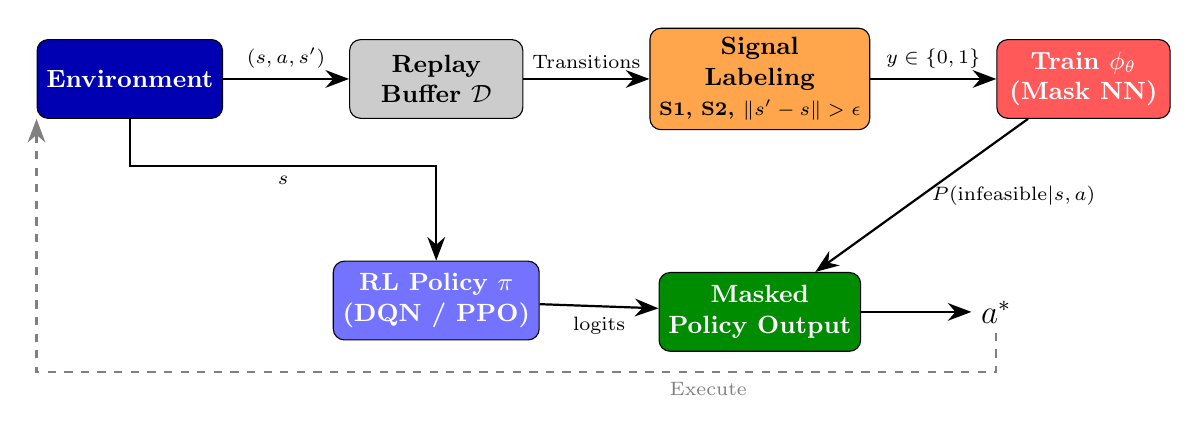
\begin{tikzpicture}[
        node distance=1.2cm and 1.6cm,
        block/.style={rectangle, draw, rounded corners, minimum height=1cm, minimum width=2.2cm, align=center, font=\small\bfseries},
        arr/.style={-{Stealth[length=3mm]}, thick},
        lbl/.style={font=\scriptsize, midway, above},
        lblb/.style={font=\scriptsize, midway, below},
    ]
        % Top row: masking pipeline
        \node[block, fill=blue!70!black, text=white] (env) {Environment};
        \node[block, fill=gray!40, right=of env] (buf) {Replay\\Buffer $\mathcal{D}$};
        \node[block, fill=orange!70, right=of buf] (sig) {Signal\\Labeling\\{\scriptsize S1, S2, $\|s'-s\|>\epsilon$}};
        \node[block, fill=red!65, text=white, right=of sig] (mask) {Train $\phi_\theta$\\(Mask NN)};

        % Bottom row: RL policy
        \node[block, fill=blue!55, text=white, below=1.8cm of buf] (policy) {RL Policy $\pi$\\(DQN / PPO)};

        % Output
        \node[block, fill=green!55!black, text=white, below=1.8cm of sig] (out) {Masked\\Policy Output};
        \node[right=1.4cm of out, font=\large\bfseries] (action) {$a^*$};

        % Arrows — top row
        \draw[arr] (env) -- node[lbl] {$(s, a, s')$} (buf);
        \draw[arr] (buf) -- node[lbl] {Transitions} (sig);
        \draw[arr] (sig) -- node[lbl] {$y \in \{0,1\}$} (mask);

        % Arrows — mask to output
        \draw[arr] (mask) -- node[right, font=\scriptsize] {$P(\text{infeasible}|s,a)$} (out);

        % Arrows — policy path
        \draw[arr] (env.south) -- ++(0,-0.6) -| node[lblb, pos=0.25] {$s$} (policy.north);
        \draw[arr] (policy) -- node[lblb] {logits} (out);

        % Output arrow
        \draw[arr] (out) -- (action);

        % Feedback loop
        \draw[arr, dashed, gray] (action.south) -- ++(0,-0.5) -| node[lblb, pos=0.15, text=gray] {Execute} (env.south west);
    \end{tikzpicture}
\end{frame}

% ============================================================================
% SLIDE 6: Related Work & Our Position
% ============================================================================
\begin{frame}{Related Work \& Our Position}
    Our work aligns most closely with \textbf{Action Masking}, but extends it substantially:

    \vspace{0.2cm}
    \begin{table}[h]
    \centering
    \small
    \begin{tabular}{p{3.2cm}p{4.5cm}p{4.5cm}}
        \toprule
        \textbf{Approach} & \textbf{How It Works} & \textbf{Limitation} \\
        \midrule
        Action Masking \newline (Wang et al.\ 2024) & Masks actions where $\|s' - s\| = 0$ & Fails on intentional waits, goal states \\
        \addlinespace
        Shielding \newline (Dey et al.\ 2023) & Predefined DFA / constraints & Requires expert prior for each env \\
        \addlinespace
        Affordances \newline (Khetarpal et al.\ 2020) & Learns preconditions for success & Typically needs expert priors \\
        \midrule
        \textcolor{contribution}{\textbf{Ours}} & \textcolor{contribution}{Environment-agnostic signals} & \textcolor{contribution}{Extends far beyond $\|s'-s\|=0$} \\
        \bottomrule
    \end{tabular}
    \end{table}

    \vspace{0.2cm}
    These approaches all restrict exploration, but rely on \textit{strict rules} or \textit{expert knowledge}. Our labeling signals are \textbf{environment-agnostic} — they require zero prior knowledge and work across any environment.
\end{frame}

% ============================================================================
% SLIDE 6: Our Contributions Overview
% ============================================================================
\begin{frame}{Our Contributions: From Simple Masking to Capability Learning}
    We extend action masking in \textbf{four key directions}:

    \vspace{0.3cm}
    \begin{enumerate}
        \item \textbf{Improved Labeling (Signal 2):} Fix the false-positive problem of base masking by detecting intentional stationarity.

        \vspace{0.15cm}
        \item \textbf{Upper-Bound Signal ($\|s' - s\| > \epsilon$):} A second base signal that masks dangerously large state transitions.

        \vspace{0.15cm}
        \item \textbf{Discounted Masking Prediction:} Learn a cumulative infeasibility function analogous to the Bellman equation — predicting infeasibility not just one step ahead, but across the entire episode.

        \vspace{0.15cm}
        \item \textbf{Model-Based RL Integration:} Use a learned world model to mask actions whose predicted trajectories lead to infeasible states $n$ steps ahead. \textit{(Novel — no prior work applies masking to model-based RL.)}
    \end{enumerate}

    \vspace{0.3cm}
    \textit{Together, these extensions form the closest proxy method to learning the true capability function $\phi$.}
\end{frame}

% ============================================================================
% SLIDE 7: Signal 1 (Base Masking)
% ============================================================================
\begin{frame}{Signal 1: Base Masking — Identity Transitions}
    The simplest signal detects actions that produce \textit{no physical effect}:

    \begin{equation}
        \text{S1:} \quad y_{\text{mask}}(s, a) =
        \begin{cases}
            1 & \text{if } \|\mathcal{T}(s, a) - s\| \leq \epsilon_{\text{low}} \\
            0 & \text{otherwise}
        \end{cases}
    \end{equation}

    \textbf{What it catches:}
    \begin{itemize}
        \item Hitting walls/boundaries $\rightarrow$ $\|s' - s\| = 0$
        \item Wind blocking weak actions $\rightarrow$ $\|s' - s\| = 0$
        \item Rain preventing upward movement $\rightarrow$ $\|s' - s\| = 0$
    \end{itemize}

    \vspace{0.3cm}
    \textbf{Failure mode:} S1 incorrectly masks \textit{intentional} stationarity:
    \begin{itemize}
        \item Agent choosing to wait (e.g., at a red light) $\rightarrow$ falsely masked
        \item Agent near the goal taking small steps $\rightarrow$ falsely masked
    \end{itemize}

    $\Rightarrow$ This motivates \textbf{Signal 2}.
\end{frame}

% ============================================================================
% SLIDE 8: Signal 2 (Improved Masking via Neighbor Consensus)
% ============================================================================
\begin{frame}{Signal 2: Neighbor Consensus — Is the Action or the State the Problem?}
    S1 flags action $a$ as stuck at state $s$ when $\|s' - s\| < \epsilon$. But \textit{is the action inherently non-moving, or is it physically blocked at this particular state?}

    \vspace{0.2cm}
    \textbf{S2 Override Rule:} Query neighboring states $\{s_1, s_2, \ldots, s_K\}$ from the replay buffer. Compute the stuck ratio for the \textit{same} action $a$ across all neighbors:
    \begin{equation}
        r(a) = \frac{\big|\{s_i : \|\mathcal{T}(s_i, a) - s_i\| < \epsilon\}\big|}{|\{s_i : \text{action } a \text{ was taken at } s_i\}|}
    \end{equation}

    \begin{equation}
        y_{\text{S2}}(s, a) =
        \begin{cases}
            0 & \text{if } r(a) > 0.99 \quad \text{(action is \textit{inherently} non-moving $\rightarrow$ un-mask)} \\
            1 & \text{if } r(a) \leq 0.99 \quad \text{(action works elsewhere $\rightarrow$ blocked here $\rightarrow$ mask)}
        \end{cases}
    \end{equation}

    \vspace{0.2cm}
    \textbf{Key insight:} If action $a$ produces $\|s'-s\| < \epsilon$ at state $s_1$ but $\|s'-s\| > \epsilon$ at neighboring state $s_2$, then $a$ \textit{can} produce movement — it is physically blocked at $s_1$, so we mask it. If $a$ \textit{never} produces movement anywhere, it is inherently designed this way (e.g., hover/wait) — so we un-mask it.
\end{frame}

% ============================================================================
% SLIDE 9: Upper-Bound Signal
% ============================================================================
\begin{frame}{Second Base Signal: Upper-Bound Masking ($\|s' - s\| > \epsilon$)}
    While S1/S2 detect actions with \textit{too little} effect, some actions produce \textit{dangerously large} state changes:

    \begin{equation}
        \text{Upper-Bound:} \quad y_{\text{upper}}(s, a) =
        \begin{cases}
            1 & \text{if } \|\mathcal{T}(s, a) - s\| > \epsilon_{\text{high}} \\
            0 & \text{otherwise}
        \end{cases}
    \end{equation}

    \textbf{Combined band-pass filter:} Only actions with \textit{moderate, controlled} effect remain unmasked:
    \begin{equation}
        y_{\text{final}}(s, a) = \mathbb{1}\big[\|s' - s\| < \epsilon_{\text{low}}\big] \;\lor\; \mathbb{1}\big[\|s' - s\| > \epsilon_{\text{high}}\big]
    \end{equation}

    \textbf{Use cases:}
    \begin{itemize}
        \item Safety-critical domains where large state jumps indicate loss of control.
        \item Robotic systems where excessive force can cause damage.
    \end{itemize}
\end{frame}

% ============================================================================
% SLIDE 10: Discounted Masking
% ============================================================================
\begin{frame}{Discounted Action Masking Prediction}
    Standard masking evaluates infeasibility \textbf{one step forward} only. We extend this to a \textbf{cumulative prediction} across the full episode:

    \begin{equation}
        \Phi(s, a) = \underbrace{\phi_{\text{immediate}}(s, a)}_{\text{one-step infeasibility}} + \gamma \cdot \underbrace{\max_{a'} \Phi(s', a')}_{\text{future cascading infeasibility}}
    \end{equation}

    This mirrors the Bellman equation for Q-values:
    \begin{equation}
        Q(s, a) = R(s, a) + \gamma \max_{a'} Q(s', a')
    \end{equation}

    \textbf{Why this matters:}
    \begin{itemize}
        \item An action may be feasible \textit{now} but leads to a state where \textit{all} actions are infeasible.
        \item $\Phi(s, a)$ captures cascading infeasibility — ``this action is fine now, but it traps me later.''
        \item $\Phi$ can be learned with the same temporal-difference machinery as $Q$.
    \end{itemize}
\end{frame}

% ============================================================================
% SLIDE 11: Model-Based RL Extension
% ============================================================================
\begin{frame}{Extension to Model-Based RL}
    To our knowledge, \textbf{no prior work applies action masking within model-based RL}.

    \vspace{0.3cm}
    \textbf{Idea:} Given a learned world model $\hat{\mathcal{T}}(s, a)$, we can simulate $n$-step rollouts and mask actions whose \textit{predicted trajectories} lead to infeasible states:

    \begin{equation}
        \hat{s}_{t+k} = \hat{\mathcal{T}}(\hat{s}_{t+k-1}, a_{t+k-1}), \quad k = 1, \ldots, n
    \end{equation}

    \begin{equation}
        y_{\text{model}}(s_t, a_t) =
        \begin{cases}
            1 & \text{if } \exists\, k \leq n : \phi(\hat{s}_{t+k}) \text{ has all actions masked} \\
            0 & \text{otherwise}
        \end{cases}
    \end{equation}

    \textbf{Advantage over $\Phi$ (Slide 10):}
    \begin{itemize}
        \item $\Phi$ requires learning a new value function via TD updates (slow).
        \item Model-based masking uses the world model to \textit{directly simulate} futures (fast, planning-time computation).
    \end{itemize}
\end{frame}

% ============================================================================
% SLIDE 12: Experimental Setup
% ============================================================================
\begin{frame}{Experimental Setup: UAV Navigation Environment}
    \begin{columns}
    \begin{column}{0.55\textwidth}
        \textbf{Environment:} 3D UAV Grid World with atmospheric dynamics.

        \vspace{0.2cm}
        \begin{itemize}
            \item \textbf{State Space} $s \in \mathbb{R}^9$:
            \begin{itemize}
                \item 3D position $(x, y, z)$
                \item Goal position $(g_x, g_y, g_z)$
                \item Wind direction $(w_x, w_y)$
                \item Rain indicator
            \end{itemize}
            \item \textbf{Action Space:} 18 discrete actions \newline (6 directions $\times$ 3 force levels)
            \item \textbf{Physical constraints:}
            \begin{itemize}
                \item Wind blocks weak-force actions
                \item Rain prevents upward movement
                \item Map boundaries
            \end{itemize}
        \end{itemize}
    \end{column}
    \begin{column}{0.4\textwidth}
        \small
        \begin{table}
        \centering
        \begin{tabular}{ll}
            \toprule
            Grid & $10 \times 10 \times 5$ \\
            Actions & 18 \\
            Max Steps & 500 \\
            Goal Reward & $+100$ \\
            \bottomrule
        \end{tabular}
        \end{table}

        \vspace{0.3cm}
        All elements (start, goal, wind zones, rain patches) are \textbf{procedurally randomized} on every episode reset to prevent memorization.
    \end{column}
    \end{columns}
\end{frame}

% ============================================================================
% SLIDE 13: Results
% ============================================================================
\begin{frame}{Results: Reward Comparison}
    \begin{figure}[h]
        \centering
        \includegraphics[width=0.5\textwidth]{reward_comparison_s1_s2_dqn.png}
        \caption{Episodic Return: Baseline DQN (grey) vs S1 Masking (cyan) vs S2 Masking (pink)}
    \end{figure}

    \begin{itemize}
        \item \textbf{S2 (pink)} converges to near-zero return significantly faster than both the baseline and S1, demonstrating that correcting false-positive masks accelerates learning.
        \item \textbf{S1 (cyan)} improves over baseline but plateaus lower — false masking of intentional stops limits its ceiling.
    \end{itemize}
\end{frame}

% ============================================================================
% SLIDE 14: Automated Threshold Discovery via GMM
% ============================================================================
\begin{frame}{Automated Threshold Discovery via GMM}
    Manually tuning $\epsilon_{\text{low}}$ and $\epsilon_{\text{high}}$ for each environment is impractical. We automate this using the agent's own experience:

    \vspace{0.2cm}
    \textbf{Observation:} The distribution of $\|s' - s\|$ is naturally \textbf{bimodal} — a cluster near zero (stuck) and a cluster with positive values (effective actions).

    \vspace{0.2cm}
    \textbf{Method:} Fit a 2-component Gaussian Mixture Model:
    \begin{equation}
        p(\|s' - s\|) = \pi_1 \cdot \mathcal{N}(\mu_{\text{stuck}}, \sigma^2_{\text{stuck}}) + \pi_2 \cdot \mathcal{N}(\mu_{\text{moved}}, \sigma^2_{\text{moved}})
    \end{equation}

    \begin{itemize}
        \item $\epsilon_{\text{low}}$ = intersection point between the two Gaussians (automatic split).
        \item $\epsilon_{\text{high}}$ = $\mu_{\text{moved}} + 2\sigma_{\text{moved}}$ (outlier detection from the ``moved'' cluster).
    \end{itemize}

    \vspace{0.2cm}
    \textbf{Result:} \textbf{Zero hyperparameters} — the thresholds are automatically discovered from the agent's own transition distribution, requiring no manual tuning and adapting to any environment.
\end{frame}

% ============================================================================
% SLIDE 15: Generalizing to More Environments
% ============================================================================
\begin{frame}{Generalizing the Approach: Moving Beyond UAV Navigation}
    Having validated Signal 1 and Signal 2 on the UAV environment, the goal is to test the framework on diverse environments.

    \vspace{0.2cm}
    \textbf{Two Key Challenges Emerged:}
    \begin{enumerate}
        \item \textbf{State-Comparison Problem:} Our current signals compute raw Euclidean distance $\|s' - s\|$ over the full state vector. In environments with mixed state semantics (e.g., a one-hot encoded taxi position vs.~a continuous velocity), this comparison becomes \textit{meaningless}.
        \vspace{0.1cm}
        \item \textbf{Future masking Problem:} Current masking is \textbf{immediate} — it only blocks an action the step it is infeasible. Ideally, the agent should learn to \textit{anticipate} infeasibility $n$ steps ahead and begin re-routing \textit{before} hitting the boundary. Moreover it should be specific to the current goal
    \end{enumerate}

    \vspace{0.2cm}
    $\Rightarrow$ Both problems point to a deeper integration of the safety signal directly into the \textbf{policy's learning objective}.
\end{frame}

% ============================================================================
% SLIDE 16: Reward-Integrated Log Penalty
% ============================================================================
\begin{frame}{A New Approach: Integrating the Log Penalty into Reward}
    \textbf{Key Insight:} The reward function already encodes discounted future consequences. If we embed the infeasibility signal inside the reward, the agent will \textit{automatically} learn to avoid stuck states $n$ steps in advance via Bellman backups.

    \vspace{0.2cm}
    \textbf{The Log Penalty Formulation:}
    \begin{equation}
        R_{\text{shaped}}(s, a, s') = R_{\text{env}}(s, a, s') + \lambda(a) \cdot \log\bigl(\|s' - s\| + \varepsilon\bigr)
    \end{equation}

    \begin{itemize}
        \item $\varepsilon$ is a small constant preventing $\log(0) = -\infty$. If $\|s'-s\| = 0$, the penalty becomes $\log(\varepsilon) \approx -11.5$ — a severe, bounded ``cliff.''
        \item $\lambda(a) \in \{0, 1\}$ is the \textbf{Signal 2 multiplier}: actions that are \textit{intentionally} stationary (e.g., \texttt{wait}, \texttt{pickup}) set $\lambda = 0$, exempting them from the penalty.
        \item The penalty is clipped to $(-\infty, 0]$ so the agent is never \textit{rewarded} for merely moving fast.
    \end{itemize}
\end{frame}

% ============================================================================
% SLIDE 17: Why Log Penalty Solves the Key Problems
% ============================================================================
\begin{frame}{Why the Log Penalty Solves Both Problems}
    \textbf{Problem 1 — State Comparison:} The $\log(\|s'-s\|)$ formulation is entirely \textbf{environment-agnostic}. It does not require a manually tuned $\epsilon$ threshold or a pre-trained offline mask. The agent's own policy generates the signal.

    \vspace{0.3cm}
    \textbf{Problem 2 — N-Step Anticipation:} This is where the approach is most powerful.
    \begin{itemize}
        \item When the agent reaches a boundary and an action produces $\|s'-s\| \approx 0$, it receives a massive negative penalty.
        \item Via \textbf{discounted reward backpropagation} (TD/Q-learning), this penalty propagates \textit{backwards} through the replay buffer to earlier states.
        \item The agent learns at an initial state: \textit{``If I take this path, I will eventually hit a penalty $n$ steps from now.''} It begins masking the action before it reaches the infeasible boundary.
    \end{itemize}

    \vspace{0.2cm}
    \textbf{Additional Benefits:}
    \begin{itemize}
        \item Eliminates the overhead of manual labeling and offline replay buffer training.
        \item The gradient of the penalty flows \textit{directly} through the policy network — the masking signal is now \textbf{end-to-end differentiable}.
    \end{itemize}
\end{frame}

% ============================================================================
% [COMMENTED OUT] SLIDE 15: The Challenge of Scale-Dependent Thresholds
% ============================================================================
%\begin{frame}{The Challenge of Scale-Dependent Thresholds}
%    \textbf{The Problem:} Raw Euclidean distance $\|s' - s\|$ is highly sensitive to the environment's coordinate scale and action magnitudes.
%    
%    \vspace{0.2cm}
%    \textbf{Example:}
%    \begin{itemize}
%        \item \textbf{Environment A:} Low, Medium, and High forces produce distances of $\{0.10, 0.20, 0.30\}$. A fixed threshold $\epsilon_{\text{low}} = 0.01$ perfectly separates ``stuck'' (0.0) from ``slow'' (0.10).
%        \item \textbf{Environment B:} The environment is scaled down, and forces produce distances of $\{0.009, 0.018, 0.027\}$.
%    \end{itemize}
%
%    \vspace{0.2cm}
%    \textbf{Consequence:} Applying the same $\epsilon_{\text{low}} = 0.01$ to Environment B causes \textbf{catastrophic over-masking}. The agent's valid ``Low'' action (0.009) is falsely flagged as ``stuck'' because $0.009 < 0.01$.
%
%    \vspace{0.3cm}
%    $\Rightarrow$ \textit{How can we formulate a generalized threshold that works seamlessly across varying environment scales?}
%\end{frame}
%
% ============================================================================
% [COMMENTED OUT] SLIDE 16: Improving State Difference via Feature Masking
% ============================================================================
%\begin{frame}{Improving State Difference via Feature Masking}
%    \textbf{The Problem:} Computing $\|s' - s\|$ over the entire state vector is susceptible to environmental noise. If a background variable (like wind direction or rain intensity) changes during the transition, the Euclidean distance will artificially inflate, even if the agent hasn't physically moved.
%    
%    \vspace{0.2cm}
%    \textbf{The Solution: State Component Masking}
%    \begin{itemize}
%        \item Instead of using the full state vector, we isolate the \textit{kinematic} or \textit{positional} components that define true movement.
%        \item \textbf{Example:} In our 11D UAV state space, we drop the environment vectors (wind, rain, goal) before computing distance:
%        \begin{equation*}
%            \text{Distance} = \|s'_{\text{xyz}} - s_{\text{xyz}}\|_{3D}
%        \end{equation*}
%        \item \textbf{Result:} The distance metric becomes perfectly robust against weather fluctuations, ensuring $\epsilon_{\text{low}}$ only measures genuine physical displacement.
%    \end{itemize}
%\end{frame}
%
% ============================================================================
% [COMMENTED OUT] SLIDE 17: Reward and Transition-Aware Distance Metrics
% ============================================================================
%\begin{frame}{Reward and Transition-Aware Distance Metrics}
%    \textbf{The Problem:} Euclidean distance alone ignores the \textit{value} of the transition. Moving $0.1$ units towards the goal is fundamentally different from moving $0.1$ units into a hazardous zone.
%    
%    \vspace{0.2cm}
%    \textbf{The Solution: Augmenting Distance with Reward Dynamics}
%    \begin{itemize}
%        \item Instead of relying solely on physical distance, we incorporate the \textbf{Reward Signal} $R(s, a, s')$ to build a stronger sense of comparison between two states.
%        \item A hybrid feasibility metric evaluates both physical and semantic progress:
%        \begin{equation*}
%            \mathcal{D}(s, s') = \alpha \|s'_{\text{xyz}} - s_{\text{xyz}}\| + \beta \big| R(s, a, s') \big|
%        \end{equation*}
%        \item \textbf{Intuition:} An action is only classified as ``stuck'' or ``infeasible'' if it produces negligible physical displacement \textit{and} fails to generate any meaningful reward. This prevents penalizing small, highly rewarding micro-adjustments near the goal.
%    \end{itemize}
%\end{frame}

% ============================================================================
% SLIDE 18: Empowerment as a Threshold-Free Signal (Future Work)
% ============================================================================
\begin{frame}{Future Signal: Empowerment as Threshold-Free Label Generation}
    \textbf{Idea:} Replace the $\epsilon$-threshold entirely with an information-theoretic measure — \textbf{Empowerment} (Klyubin et al. 2005, Salge et al. 2014):
    \begin{equation}
        E(s) := I(a;\; s' \mid s) \quad \text{(mutual information between action and next state)}
    \end{equation}

    \textbf{Intuition:} If \textit{all} actions at state $s$ lead to the \textit{same} next state $s'$, then the agent has \textbf{zero empowerment} — any input signal through actions produces the same output. The agent has no control over its environment at this state.

    \vspace{0.2cm}
    \textbf{Per-action empowerment} (variance approximation, Gregor et al. 2016):
    \begin{equation}
        \hat{E}_j(s) := \text{Var}_{a_j \sim \text{Uniform}}[\mathcal{T}(s, a)] \approx 0 \implies \text{action } j \text{ is infeasible at } s
    \end{equation}

    \vspace{0.2cm}
    \textbf{Advantage:} No $\epsilon$ threshold needed — empowerment is a \textit{continuous} measure of capability. $\hat{E}_j(s) \approx 0$ directly indicates infeasibility without any manual calibration. This can serve as an additional label generation criterion alongside our $\epsilon$-based signals.
\end{frame}

% ============================================================================
% SLIDE 19: Continual RL Application
% ============================================================================
\begin{frame}{Application: Capability Transfer in Continual RL}
    In continual RL, the environment or task changes over time. Standard RL must relearn \textit{everything} from scratch. But physical capabilities rarely change:

    \vspace{0.2cm}
    \begin{table}[h]
    \centering
    \small
    \begin{tabular}{p{4cm}p{2.5cm}p{5.5cm}}
        \toprule
        \textbf{Knowledge Type} & \textbf{Changes?} & \textbf{Example} \\
        \midrule
        Reward structure & Yes (new tasks) & ``Navigate to Goal B instead of A'' \\
        Physical capabilities & Rarely & ``I still cannot fly through walls'' \\
        \bottomrule
    \end{tabular}
    \end{table}

    \textbf{Why $\phi$ is a game-changer for Continual RL:}
    \begin{enumerate}
        \item \textbf{Capability Transfer:} When the task changes, reset $Q$-network but \textit{keep} $\phi_\theta$. The agent instantly avoids re-exploring known-infeasible actions $\Rightarrow$ dramatic sample savings.
        \item \textbf{Drift Detection:} When dynamics change (e.g., joint degradation), $\phi$ detects it \textit{before} the reward drops — previously feasible actions start producing $\|s'-s\| < \epsilon$.
        \item \textbf{Safety Memory:} $\phi_\theta$ is a separate network from the policy. Even as $Q$-network adapts to new tasks, $\phi$ preserves the agent's understanding of physical limits — preventing catastrophic forgetting of safety.
    \end{enumerate}
\end{frame}

% ============================================================================
% SLIDE 20: The Big Picture
% ============================================================================
\begin{frame}{The Big Picture: Closest Proxy to Learning Capabilities}
    \textbf{Thesis:} While learning the true capability function $\phi$ directly is intractable, our combined ideas offer the \textbf{closest proxy method}:

    \vspace{0.3cm}
    \begin{enumerate}
        \item \textbf{S1 + S2:} Agnostic labeling signals that detect infeasibility from raw transitions — no expert knowledge required.
        \item \textbf{$\|s'-s\| > \epsilon$:} Upper-bound signal capturing dangerously excessive effects.
        \item \textbf{$\Phi(s, a)$:} Discounted masking extends capability assessment from one-step to the full episode horizon.
        \item \textbf{Model-Based Integration:} World model enables $n$-step lookahead masking at planning time.
    \end{enumerate}

    \vspace{0.3cm}
    Some of these ideas exist in isolation in prior work. \textbf{Our contribution} is (a) improving the base signals (S2), (b) the Bellman-style discounted extension, (c) model-based integration, and (d) framing all of this under the unifying goal of \textit{learning capabilities}.
\end{frame}

% ============================================================================
% SLIDE 21: Conclusion & Future Scope
% ============================================================================
\begin{frame}{Conclusion \& Future Scope}
    \textbf{Contributions to date:}
    \begin{itemize}
        \item Defined the capability function $\phi_\theta: \mathcal{S} \rightarrow \mathbb{R}^{|\mathcal{A}|}$ as a unifying abstraction.
        \item Improved action masking signals (S1 $\rightarrow$ S2) with empirical validation.
        \item Proposed Bellman-style discounted masking $\Phi(s, a)$.
        \item Identified model-based RL as a novel application domain for masking.
    \end{itemize}

    \vspace{0.3cm}
    \textbf{Connection to Safe RL:}
    \begin{itemize}
        \item Action masking heavily overlaps with \textit{Shielding} and \textit{Safe RL}.
        \item Our approach acts as \textbf{agnostic, unconstrained safety} — no predefined constraints needed.
        \item \textbf{Future:} Detailed experiments combining our agnostic masking with traditional Safe RL algorithms (CPO, TRPO-Lagrangian) to measure compound performance gains.
    \end{itemize}
\end{frame}

\end{document}
